\documentclass[11pt,letterpaper]{article}
\usepackage{fullpage}
\usepackage{amsmath}
\usepackage{amsfonts}
\usepackage{amssymb}
\usepackage{amsthm}
\usepackage{array}
\usepackage[dvipsnames]{xcolor}
\usepackage{textcomp}
\usepackage{graphicx}

\newcommand{\N}{\mathbb{N}}
\newcommand{\R}{\mathbb{R}}
\newcommand{\floor}[1]{\left\lfloor{#1}\right\rfloor}

\newenvironment{solution}{\color{Violet}\textit{Solution.}}{\color{black}}

\begin{document}
\begin{center}
    \begin{large}
        \textbf{Homework 4} \\
        MAD6206 \\
        Carson Mulvey
    \end{large}
\end{center}

\color{black}

\begin{enumerate}
    \item[12.10.8.] Calculate the Möbius functions of the posets whose Hasse diagrams appear in Fig. 12.1.
    \begin{figure}[h]
        \centering
        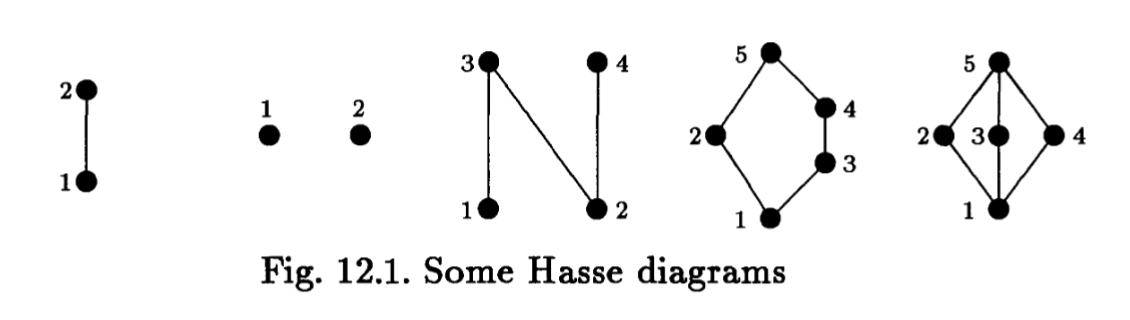
\includegraphics[width=8cm]{figure.png}
    \end{figure}
    
    \begin{solution}
        \begin{enumerate}
            \item $\mu(1,1) = \mu(2,2) = 1$, $\mu(1,2) = -1$, $\mu(2,1) = 0$
            \item $\mu(1,1) = \mu(2,2) = 1$, $\mu(1,2) = \mu(2,1) = 0$
            \item \[[\mu] = \left[ {\begin{array}{cccc}
                1 & 0 & -1 & 0\\
                0 & 1 & -1 & -1\\
                0 & 0 & 1 & 0\\
                0 & 0 & 0 & 1\\
  \end{array} } \right]\]
            \item \[[\mu] = \left[ {\begin{array}{ccccc}
                1 & -1 & -1 & 0 & 1\\
                0 & 1 & 0 & 0 & -1\\
                0 & 0 & 1 & -1 & 0\\
                0 & 0 & 0 & 1 & -1\\
                0 & 0 & 0 & 0 & 1\\
  \end{array} } \right]\]
  \item \[[\mu] = \left[ {\begin{array}{ccccc}
    1 & -1 & -1 & -1 & 2\\
    0 & 1 & 0 & 0 & -1\\
    0 & 0 & 1 & 0 & -1\\
    0 & 0 & 0 & 1 & -1\\
    0 & 0 & 0 & 0 & 1\\
  \end{array} } \right]\]
        \end{enumerate}
    \end{solution}

    \item[12.10.10.] Let $a,b$ be elements of a poset $P$. Prove that $\mu(a,b)=\sum_{i\geq 0}(-1)^ic_i$, where $c_i$ is the number of chains
    \[  a = x_0 < \dots < x_i = b.  \]

    \begin{solution}
        We can replace $c_i$ with the notation $c(r,i)$, which represents the number of chains
        \[  a = x_0 < \dots < x_i = r,  \]
        for any element $a \leq r \leq b$.

        \textbf{Lemma.} For elements $a,b$, with $i>0$,
        \[
            c(b,i+1) = \sum_{a \leq r < b} c(r,i).
        \]
        \textit{Proof.} Consider a chain from $a$ to $b$ where
        \[ a = x_0 < \dots < x_i < x_{i+1} = b. \]
        Removing $b$ from this chain produces a chain
        \[ a = x_0 < \dots < x_i = r.\]
        Conversely, a chain from $a$ to $r$ of length $i+1$ can be extended to $b$, creating a chain of length $i+2$. Thus, we have a bijection between chains of length $i+2$ from $a$ to $b$ (LHS), and chains from $a$ to $r$ of length $i+1$ for all possible $r$ (RHS). (end of Lemma)

        For two elements $a,b$, let $H$ be the maximal $i$ such that $c(b,i)$ is nonzero. We will prove by strong induction on $H$. For $H=0$, we have $a=x_0=b$, and $\mu(a,b) = \sum_{i\geq 0}(-1)^ic(b,i) = 1$, as desired. Now consider elements $a\neq b$ where $H=K>0$. For some element $r$ with $a \leq r < b$, we have $H < K$ between $a$ and $r$, as all chains are smaller than the maximal chain from $a$ to $b$. By our inductive hypothesis, we have
        \[  \mu(a,r)=\sum_{i\geq 0}(-1)^ic(r,i). \tag{$\ast$}   \] 
        By the recursive formula for the Möbius function, we have
        \[    \mu(a,b) = -\sum_{a \leq r < b} \mu(a,r). \]
        But ($\ast$) implies
        \begin{align*}
            \mu(a,b) &= \sum_{a \leq r < b} \sum_{i \geq 0} (-1)^{i+1}c(r,i) \\
            &= \sum_{i \geq 0} \sum_{a \leq r < b} (-1)^{i+1}c(r,i) \\
            &= \sum_{i \geq 0} (-1)^{i+1} \sum_{a \leq r < b}c(r,i) \\
            &= \sum_{i \geq 0} (-1)^{i+1} c(b, i+1) \qquad\text{(by Lemma)}\\
            &= \sum_{i \geq 1} (-1)^{i} c(b, i).
        \end{align*}
        But $(-1)^0c(b,0)=0$ when $a\neq b$, so
        \[
            \mu(a,b) = \sum_{i \geq 0} (-1)^{i} c(b, i),
        \]
        as desired. \qed


    \end{solution}

    \item[Non-book 1.] Prove that a poset of size $mn+1$ has a chain of size greater than $m$ or an antichain of size greater than $n$.
    
    \begin{solution}
        Let poset $P$ have no antichain with greater than $n$ elements. Then let the maximum antichain size (i.e. the width) of $P$ be $a\leq n$. By Dilworth's Theorem, the number of elements in a minimal chain cover is also $a$. Then by the Pigeonhole Principle, at least one chain in any chain cover must contain at least $\left\lceil \frac{mn+1}{a} \right\rceil$ elements. But since $a\leq n$, we have 
		\begin{align*}
			\left\lceil \frac{mn+1}{a} \right\rceil &\geq 
            \left\lceil \frac{mn+1}{n} \right\rceil \\ &= 
            \left\lceil m+\frac{1}{n} \right\rceil \\
			&= m+1.
		\end{align*}
		Thus, $P$ contains a chain with greater than $m$ elements. \qed
    \end{solution}
    
    \item[Non-book 2.] Prove that $I$ is an ideal if and only if it is an initial segment of some linear extension of $P$. 
    
    \begin{solution}
        ($\Rightarrow$) The case of $I=P$ is clear, so consider $I \neq P$. We can create linear extensions $f_1\colon I \rightarrow [|I|]$ on $I$ as a subposet and $f_2\colon P\backslash I \rightarrow \{|I|+1,\dots,|P|\}$ on $P\backslash I$ as a subposet. Such linear extensions must exist as both subposets are nonempty. Then define $f\colon P \rightarrow [|P|]$ by mapping $x\in P$ to $f_1(x)$ if $x\in I$ and $f_2(x)$ otherwise. We then claim that $f$ is a valid linear extension of $P$. To see this, we take elements $x,y$ in $P$ with $x\leq y$. If $x,y\in I$ or $x,y\notin I$, then $f(x)\leq f(y)$ by definition of $f_1$ and $f_2$, respectively. If $x\in I$ and $y \notin I$, then $f(x)\leq f(y)$ is clear by comparing the codomains of $f_1$ and $f_2$. Finally, $y \in I$ and $x \notin I$ is not possible, as $x\leq y$ implies $x \in I$ by definition of an ideal. Thus, $f$ is a linear extension with $I$ as its initial segment.

        ($\Leftarrow$) Let $I$ be the initial segment of a linear extension $f$ on $P$. Let $x\in I$. If $y \leq x$, then $f(y) \leq f(x)$ by definition of a linear extension. This implies that $y$ is also in the initial segment of $f$, i.e. $y \in I$. Thus, $I$ is an ideal. \qed
    \end{solution}
    
    \item[Non-book 3.] Let $L$ be a finite poset with a maximum element $\hat{1}$ such that every two elements have a meet. Prove that $L$ is a lattice.
    
    \begin{solution}
        Let $x,y \in L$. Define $\mathcal{B} = \{b \in L \colon x,y \leq b\}$. We note that $\hat{1} \in \mathcal{B}$, so $\mathcal{B}$ is nonempty. We enumerate $\mathcal{B} = \{b_1,b_2,\dots,b_k\}$. We then consider the meet of all $b_i$,
        \[
        m = \bigwedge_{i=1}^k b_i.
        \]
        We claim that the join of $x$ and $y$ exists, namely $x\vee y = m$. Since $x,y \leq b_i$ for all $i$, $x$ and $y$ are at most as large as the common lower bound of all $b_i$. Thus, $x,y \leq m$, and $m \in \mathcal{B}$. Moreover, for all $i \in [k]$, we have $m \leq b_i$, which implies $m = \min \mathcal{B}$. Thus $x\vee y = m$, as desired. \qed
    \end{solution}

\end{enumerate}

\end{document}